%!TEX root = ../report.tex
%%%%%%%%%%%%%%%%%%%%%%%%%%%%%%%%%%%%%%%%%%%%%%%%%%%%%%%%%%%%%%%%%%%%%%%
%%%%%%%%%%%%%%%%%%%%%%%%%%%%%%%%%%%%%%%%%%%%%%%%%%%%%%%%%%%%%%%%%%%%%%%
%%%%%                                                                 %
%%%%%     architecture.tex                                            %
%%%%%                                                                 %
%%%%% Author:      Florian Zaruba                                     %
%%%%% Created:     <date>                                             %
%%%%% Description: <description>                                      %
%%%%%                                                                 %
%%%%%%%%%%%%%%%%%%%%%%%%%%%%%%%%%%%%%%%%%%%%%%%%%%%%%%%%%%%%%%%%%%%%%%%
%%%%%%%%%%%%%%%%%%%%%%%%%%%%%%%%%%%%%%%%%%%%%%%%%%%%%%%%%%%%%%%%%%%%%%%

\chapter{Hardware Architecture}

In this chapter I will give an architectural overview of the \pulpino SoC. As described in the instructional chapter both cores available for \pulpino feature a 32-bit 4-stage in order pipeline with distinct ports to the instruction and data RAMs. Since the cores are totally pin compatible one can swap them as needed without modifying any RTL.

\pulpino uses a 32-bit wide AXI as its main interconnect. The memories and the core itself are connected to the AXI Bus via dedicated bus adapters. The APB peripherals are connected to the AXI bus through a AXI2APB adapter. As all components withing the system have access to the AXI bus they share a common memory map. This makes it particularly easy to write and read registers from each peripheral, the core and memories' content. The overall device architecture is depicted in figure~\ref{fig:block_diagram}.


\begin{figure}[tbph]
  \centering
  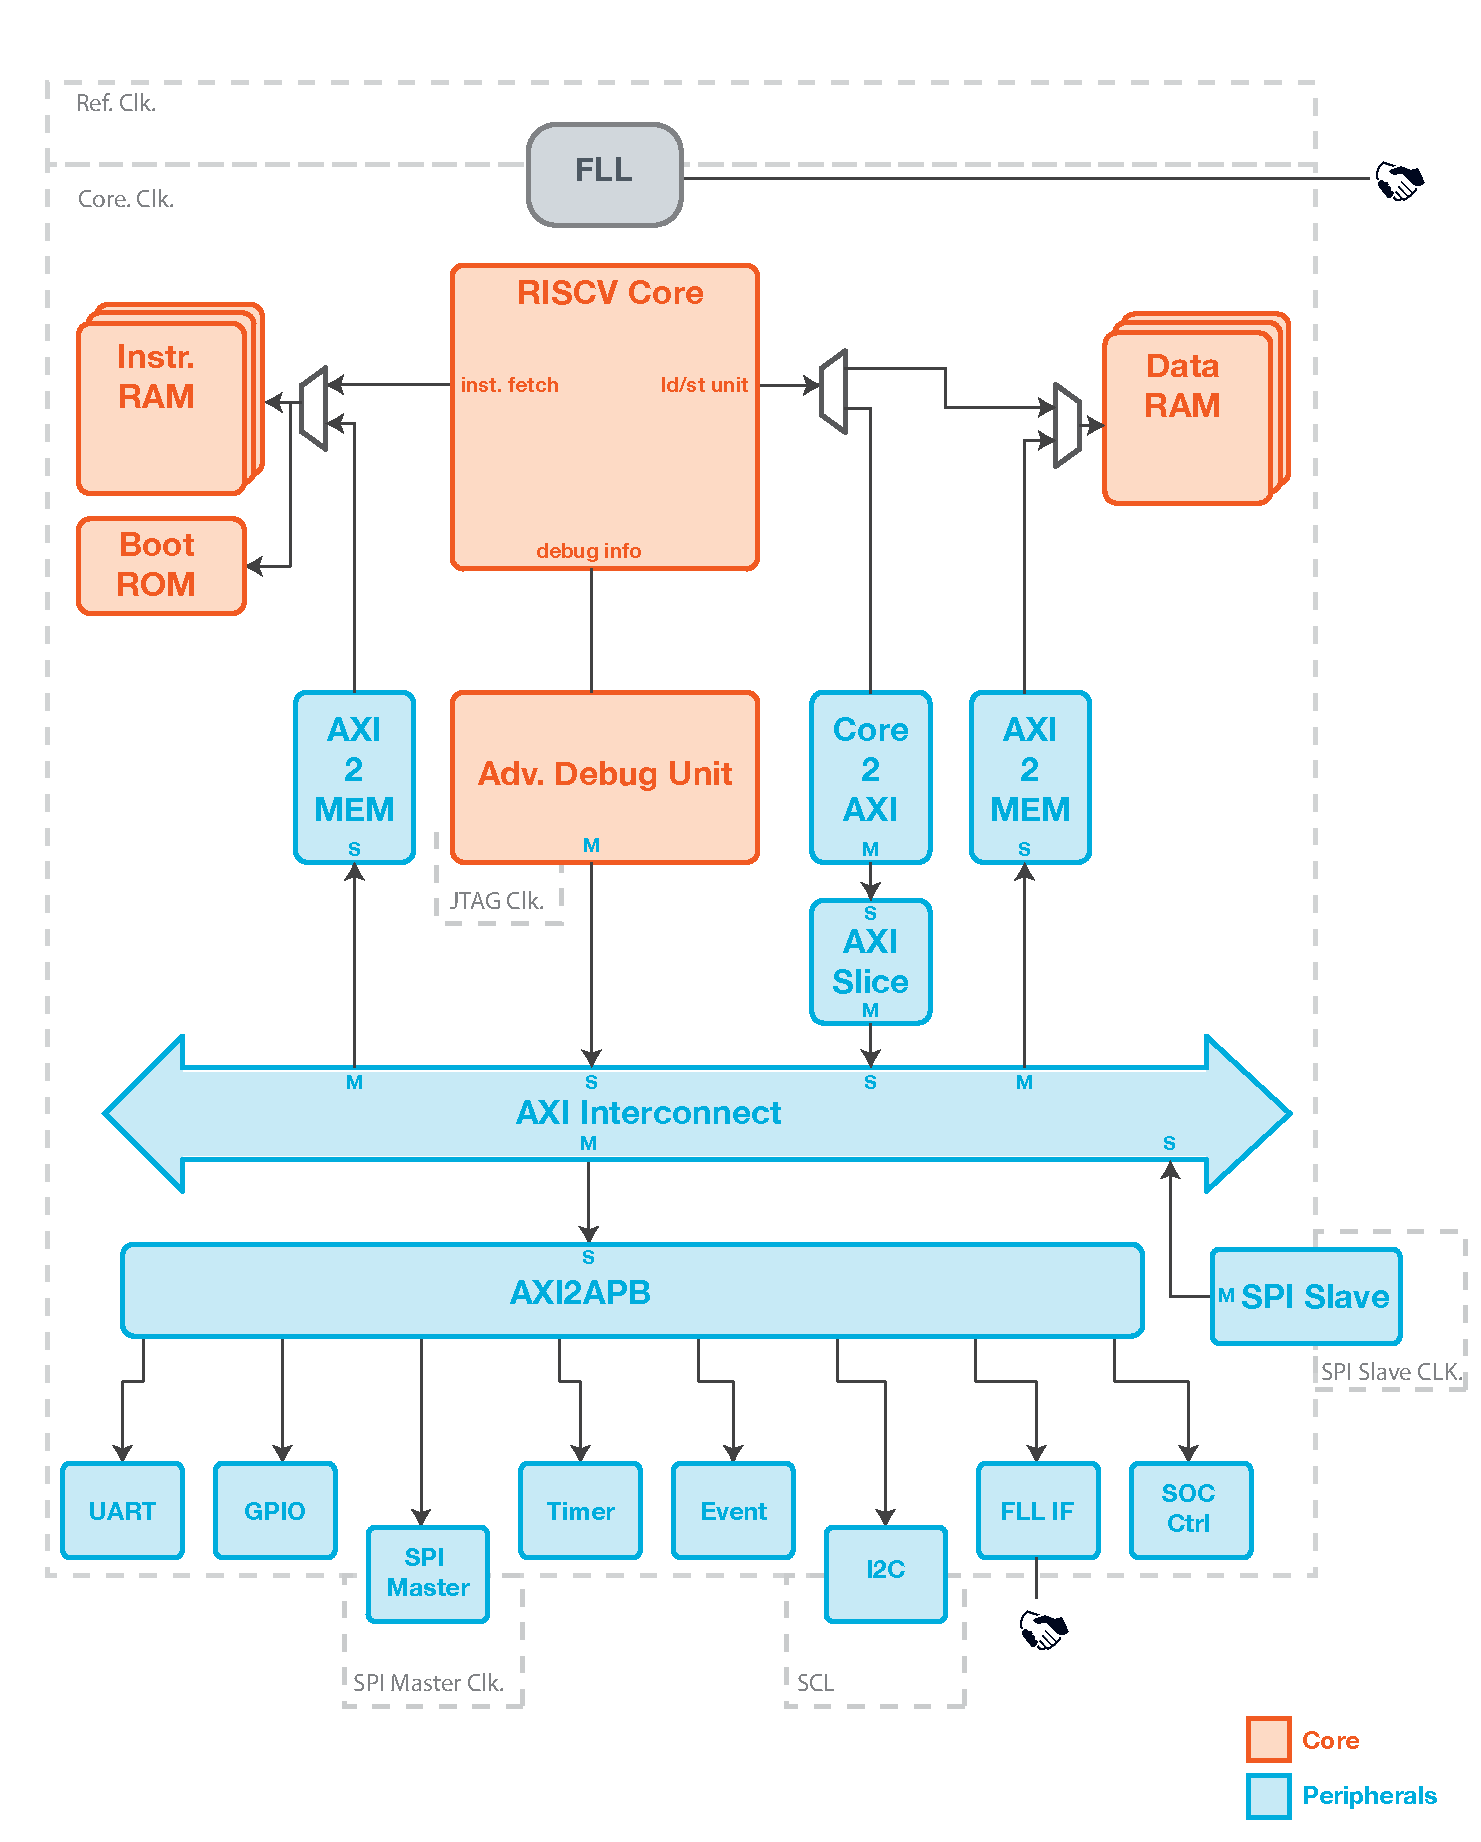
\includegraphics[width=\linewidth]{./figures/pulpino_blockdiagram}
  \caption{\pulpino block diagram}
  \label{fig:block_diagram}
\end{figure}


\section{Core}

\pulpino comes with two cores available. Both cores have been developed by the PULP group. This can either be the RISC-V core RI5CY or the pin compatible OpenRISC core OR10N.

\subsection{OpenRISC - OR10N}

OR10N was developed as part of a semester thesis here at IIS by Renzo Andri and Matthias Baer in 2014. It was meant to replace the former OpenRISC 1200 core used for the PULP project. The core employs a 32-bit 4 Stage in-order pipeline and has shown to be significantly faster then the reference implementation of the OpenCores community called OpenRISC 1200 \cite{renzobaer}.

\subsection{RISC-V - RI5CY}

RI5CY is a 4-stage in-order CPU based on the freely available RISC-V instruction set developed at UCB. The core has been mainly developed by Sven Stucki as part of his master's thesis (TODO: Citiation??). RI5CY is loosely based on OR10N. 

The RISC-V instruction set comes in a very modular and extendable flavor \cite{Waterman:EECS-2014-54}:

\begin{itemize}
    \item \textbf{RV32I}, \textbf{RV64I}: Is the 32-bit or 64-bit respectively, base integer instruction set. It describes general instruction formats and includes all operations to modify (integer) data and control flow. We fully support the bas integer instruction set with our RI5CY core.
    \item \textbf{M Standard Extension}: The M standard extension describes multiplication and division operations that multiply or divide values held in two integer registers. We provide only partial support for the M extension since our current multiplier implementation uses a single-cycle 32 bit lower result multiplier. As a matter of fact we do not support divisions and multiplications that return the upper half of the result.
    \item \textbf{A} (Atomic), \textbf{F} (single precision floating point) and \textbf{D} (double precision floating point) \textbf{standard extension}: We currently do not support any of these extensions.
    \item \textbf{C standard compressed ISA}: The compressed ISA specification is currently a proposal but will likely be frozen in the near future. The compressed ISA aims to reduce static and dynamic code size by adopting a simple compression scheme (i.e. small immediate values, one of the registers is the zero register $x0$,...). According to the current compressed ISA draft specification typically 50\%-60\% of the RISC-V instructions in a program can be replaced with RVC instructions, resulting in a 25\%-30\% code-size reduction~\cite{Waterman:EECS-2015-209}.
\end{itemize}

In addition the RISC-V ISA provides the opportunity to define instruction set extensions that are not currently officially supported. We do make particular use of this with support of post-increment load and store instructions, hardware loops and packed-SIMD instructions.


\section{AXI Interconnect}

\pulpino features an AXI bus as its main interconnect. Memories and the core are connected via dedicated bus adapters developed by the PULP group. The main advantage of having everything sharing one interconnect is the fact that the whole architecture becomes memory mapped.

\subsection{AXI Slices}

The AXI interconnect can be sliced when becoming necessary. This means that registers are getting inserted at the specified position. This can be of help if timing on certain parts of the interconnect becomes tight. Slicing the interconnect comes at the price of loosing one clock cycle (of course depending on the number of slices inserted) upon access to this certain part of the interconnect. In the present \pulpino design this was necessary between the core bus adapter and the bus itself due the criticality of that path.


\subsection{SPI Slave}
\label{subsec:spi_slave}

The SPI Slave is a special peripheral in the sense that it allows to receive and send data without any interaction of the core itself. This allows us to treat \pulpino as a normal SPI Slave that can get its whole memory region written from an external SPI Master (for example another microcontroller). This has the advantage that we can pre-load its entire memorie region (therefore writing all RAMS and arbitrary configuration registers). This features is inherited from PULP that was designed with the goal in mind that it will almost always be used in the context of an external host environment. Hence this provides us with another way of booting \pulpino.

The SPI Slave has an AXI master through which it can access the whole memory region. It can be either used as a standard SPI Slave or as an Quad SPI which takes four bi-directional data lanes and provides four times the data throughput compared to normal SPI.

If you plan for an ASIC implementation you may want to reduce the pin count by only using standard SPI. 

\subsection{Memory and Core adapters}

We provide special memory and core adapters which are hooked up to the AXI bus. This allows us to read and write all memories through AXI. In particular this can be useful when loading a program (see~\ref{subsec:spi_slave}) or testing the memories.

\section{Advanced Debug Unit}

The advanced debug unit (ADU) originates from an OpenCores project. It has been adapted by us for the use in the PULP project. On the one side the ADU interfaces the core with a custom made debug interface that is the same for the OR1ON and RI5CY core and an interface to the AXI Bus. On the other hand it provides a JTAG TAP (Test Access Port) that can be interfaced by the standard JTAG protocol.

With the ADU it is possible to debug the core by a software debugger such as GDB running on a separate host PC.

The ADU is designed with different modules in place. On the one hand side it the JTAG TAP module that implements the JTAG protocol and on the other hand we have a module for the AXI and one module for the core. Each module must be dedicatedly activated before it can be used.

Sub-modules generally consist of two parts: internal registers, and a bus interface. Internal module registers may contain information about the status of the module (such as the error register in the AXI4 module), or they may control external I/O lines (such as the reset and stall lines from the OR1ON module). Each sub-module using one or more registers contains an index register, which enables one internal register at a time for reading or writing. Internal registers are selected, read, and written by sending commands to a sub-module through the TAP.


\section{APB Peripherals}

\subsection{Interrupt and Sleep Unit}

The unit is conducted as an APB peripheral. Each interrupt can be enabled or disabled and can have its pending status set or cleared by software (resulting in the fact that we support "soft interrupts"). The units main purpose is to keep track of all arriving interrupts and outputting the interrupt with the highest priority (starting from 0 up to 31) - iff it is enabled -  to the core in a one-hot encoded fashion. 

The interrupt unit can basically handle two types of interrupt sources:

\begin{itemize}
    \item \textbf{Pulsed interrupt request} - the interrupt request is at least one clock cycle long. When the interrupt controller receives a pulse at its interrupt input, the pending status is set and held until the interrupt gets served.
    \item L\textbf{evel triggered interrupt request} - the interrupt source holds the request high until the interrupt is serviced.
\end{itemize}

The interrupt output to the core is level sensitive. As long as there is a pending interrupt the corresponding interrupt request line (\verb+irq_o+) gets asserted. If the core wants to acknowledge an external interrupt it needs to clear the corresponding pending interrupt by writing 1 to the \verb+clear_pending+ (ICP) register. The interrupt is then de-asserted.

The event unit has exactly the same RTL layout as the interrupt unit. The only difference is that its \verb+signal_o+ is not forwarded to the processor core. An event can wake the core from sleep state. (TODO: provide a facility to get the currently pending event).

The sleep unit's task is to put the core into a low power mode by disabling its clock (through a clock gate). It therefore needs to track the sleep status of the core through a simple FSM (see figure~\ref{fig3}). The sleep unit is tightly coupled to the interrupt unit since it needs to wake the processor if an enabled interrupt arrives.
The sleep controller is as well conducted as an APB peripheral with two registers (see figure~\ref{fig4}):

\begin{enumerate}
    \item \textbf{Sleep Controll Register:} By writing the lowest bit (SE - Sleep Enable) to 1 the core requests to be put to sleep. Upon wakeup this bit is cleared by the controller.
    \item \textbf{Sleep Status Register:} This register contains the current sleep status of the core. This is helpful if for example you want to get the sleep status through the debug interface. Writes to this location are ignored.
\end{enumerate}

If the core signals that it is idle and wants to be put to sleep it writes the SE register. The controller then enters the \verb+SHUTDOWN+ state where the fetch enable signal of the core is de-asserted and no more instructions are fetched. After the processor has flushed its pipeline (signaled by a low \verb+core_busy+ signal) its clock is gated and the \verb+SLEEP+ state is entered. It now resides in a lower power state and can only be waked up by an external interrupt event (\verb+signal_i+ asserted).

Because the interrupt unit has control over the fetch enable signal of the core it has been immediately suggested itself to put the fetch enable synchronizer into the event unit as well. Because the event unit is clock gated after reset by \pulpino peripheral (\ref{subsec:pulpino_peripheral}) it was necessary to also include a clock signal that is not clock gated.

\subsection{Timer Unit}

The timer provides a facility to cycle accurately time certain events and/or trigger interrupts or events respectively. In detail it should be possible to generate a timer overflow interrupt/event if the timer reaches its highest value and a timer output compare event when the timer is equal to a certain value set in the timer output compare register.


Additionally a timer control register makes it possible to set a pre-scaler, enable/disable timer overflow and timer output compare interrupts/events and to start and stop the timer respectively.

\subsection{\pulpino peripheral}
\label{subsec:pulpino_peripheral}

In order to control certain features of the SoC a special set of control registers is needed to do so. Since this is highly application specific (e.g. it only applies to this distinct SoC configuration) it has been my indention to logically and physically separate this sort of functionality into an independent peripheral.

This peripheral has control over the following registers:
\begin{itemize}
  \item Control of all pads with double functionality: Whether they should be used as GPIO or perform there special function like SPI, UART, etc. The default value is set so that the special function is activated. For further information on how the pads are configured refer to table~\ref{tab:pads}.
  \item Control of peripheral clock gating: In order to save energy most of the peripherals are clock gated by default. Actually the only exception to this is the \pulpino peripheral itself. To activate the desired peripheral you have to set the corresponding bit in the clock gating register.
  \item Boot address: The register manages the boot address from which the core start fetching its instructions once the fetch enable signal has become asserted.
  \item Version String: This peripheral provides a hard coded version string that represents part of the current configuration which is especially crucial for the ASIC implementation. The version string contains basic information about the system's configuration like RAM and ROM sizes and whether there are instruction and data caches in place:

  \begin{bytefield}[rightcurly=.,endianness=big]{32}
  \bitheader{31,0} \\
  \begin{rightwordgroup}{Version Register}
    \bitbox{4}{0000}
    \bitbox{1}{D}
    \bitbox{1}{I}
    \bitbox{5}{Version}
    \bitbox{8}{Instr. RAM}
    \bitbox{8}{Data RAM}
    \bitbox{5}{Version}
  \end{rightwordgroup}
  \end{bytefield} 
  For a detailed explanation about the single bitfields please refer to register description in~\ref{sec:register_map}.
  \item Pad configuration: For the pad's primary function the peripheral controls the configuration parameters like slew rate, drive strength and pull-ups. For a list of all reset values refer to~\ref{tab:pads}. 
\end{itemize}


\subsection{GPIO}
\label{subsec:gpio_peripheral}

General prupose input output is managed through this dedicated peripheral. It controls whether the signal is an input or an output. In addition it allows you to configure the pads according to your needs, similar to the \pulpino peripheral does for specialized I/O. Furthermore the GPIO peripheral can trigger interrupts when the level of a pad is changing.

\subsection{I2C}

I2C (Inter-Integrated Circuit) is a serial bus interface invented by Philips Seminconductor. It is typically used for communication with lower-speed ICs like for example an EEPROM on a printed circuit board (PCB).

I2C uses two bidirectional open-drain lines called Serial Data Line (SDA) and Serial Clock Line (SCL) pulled up. It supports multi-master and multi-slave bus systems. Arbitration in multi-master clock gets done by specifiying bus access schemes so that no more than one master is accessing the bus at once.

In our I2C implementation the clock is derived from the main system clock by setting an appropriate prescaler value. The current status of the I2C peripheral is held in the corresponding status register. Dpending on the value of the command register the I2C performs a different operation. This can either be a start, stop, read and write operation depending on the bit set in the command register. 

The control register allows you to enable interrupts. The interrupt flag can also be polled from the status register in case interrupts are not enabled. In addition interrupts get generated when either the transmission has been successful or bus arbitration has been lost. The interrupt needs to be cleared in the event unit as well as in the I2C peripheral by writing 0x01 to the command register. For a detailed explanation of the registers refer to the register description in the appendix~\ref{sec:register_map}. 

\subsection{UART (Universal Asynchronous Receiver Transmitter)}

A universal asynchronous receiver/transmitter (UART) is piece of hardware that translates data between parallel and serial forms. It was frequently found in former times as part of the RS-232 interface of personal computers but is still widely incorporated on micro controller platforms. This UART is mostly based on the 16750 UART developed by Texas Instruments (TI) and was written by Sebastian Witt for the OpenCores project. It is distributed under a LGPL license. 

The design is pin and register compatible to TI's 16550/16750 UART. It allows for variable baud generation based on the main system clock. It supports the following features:

\begin{itemize}
    \item Full synchronous design
    \item Pin compatible to 16550/16750
    \item Register compatible to 16550/16750
    \item Baudrate generator with clock enable
    \item Supports 5/6/7/8 bit characters
    \item None/Even/Odd parity bit generation and detection
    \item Supports 1/1.5/2 stop bit generation
    \item 16/64 byte FIFO mode
    \item Receiver FIFO trigger levels 1/4/8/14/16/32/56
    \item Control lines RTS/CTS/DTR/DSR/DCD/RI/OUT1/OUT2
    \item Automatic flow control with RTS/CTS
    \item All interrupts sources/modes 
\end{itemize}


\subsection{SPI Master}

\subsection{FLL Interface}

\section{FLL}







